\chapter{Introduction}
\label{chapter1}

\section{Overview}
In the last decades industry is being moving from the use of traditional robotic arms (manipulators), which executes highly specific simple tasks in controlled and secure environments, like spot welding, towards more complex and flexible robotic systems, which should be able to cope with dynamic and uncertain environments. \\ 
Even before industrial robot manipulators, in the '50s, the idea of building mobile systems that can move autonomously in unstructured environments was raising. The first was William Grey Walter who built a couple of mobile vehicles with already embedded sensors to avoid obstacles, then in 1969 the mobile robot SHAKEY has been develoed in Stanford University, named after its shaking behaviour to move towards an object which it could recognise, then the JPL Rover for space exploration has been developed in the '70s, and so on until nowadays where different types of robots can be found in a great variety of environments, ranging from the cleaning robots in people houses, to legged mobile robots inspired to animal behaviour.
\begin{figure}[h!]
	\centering
	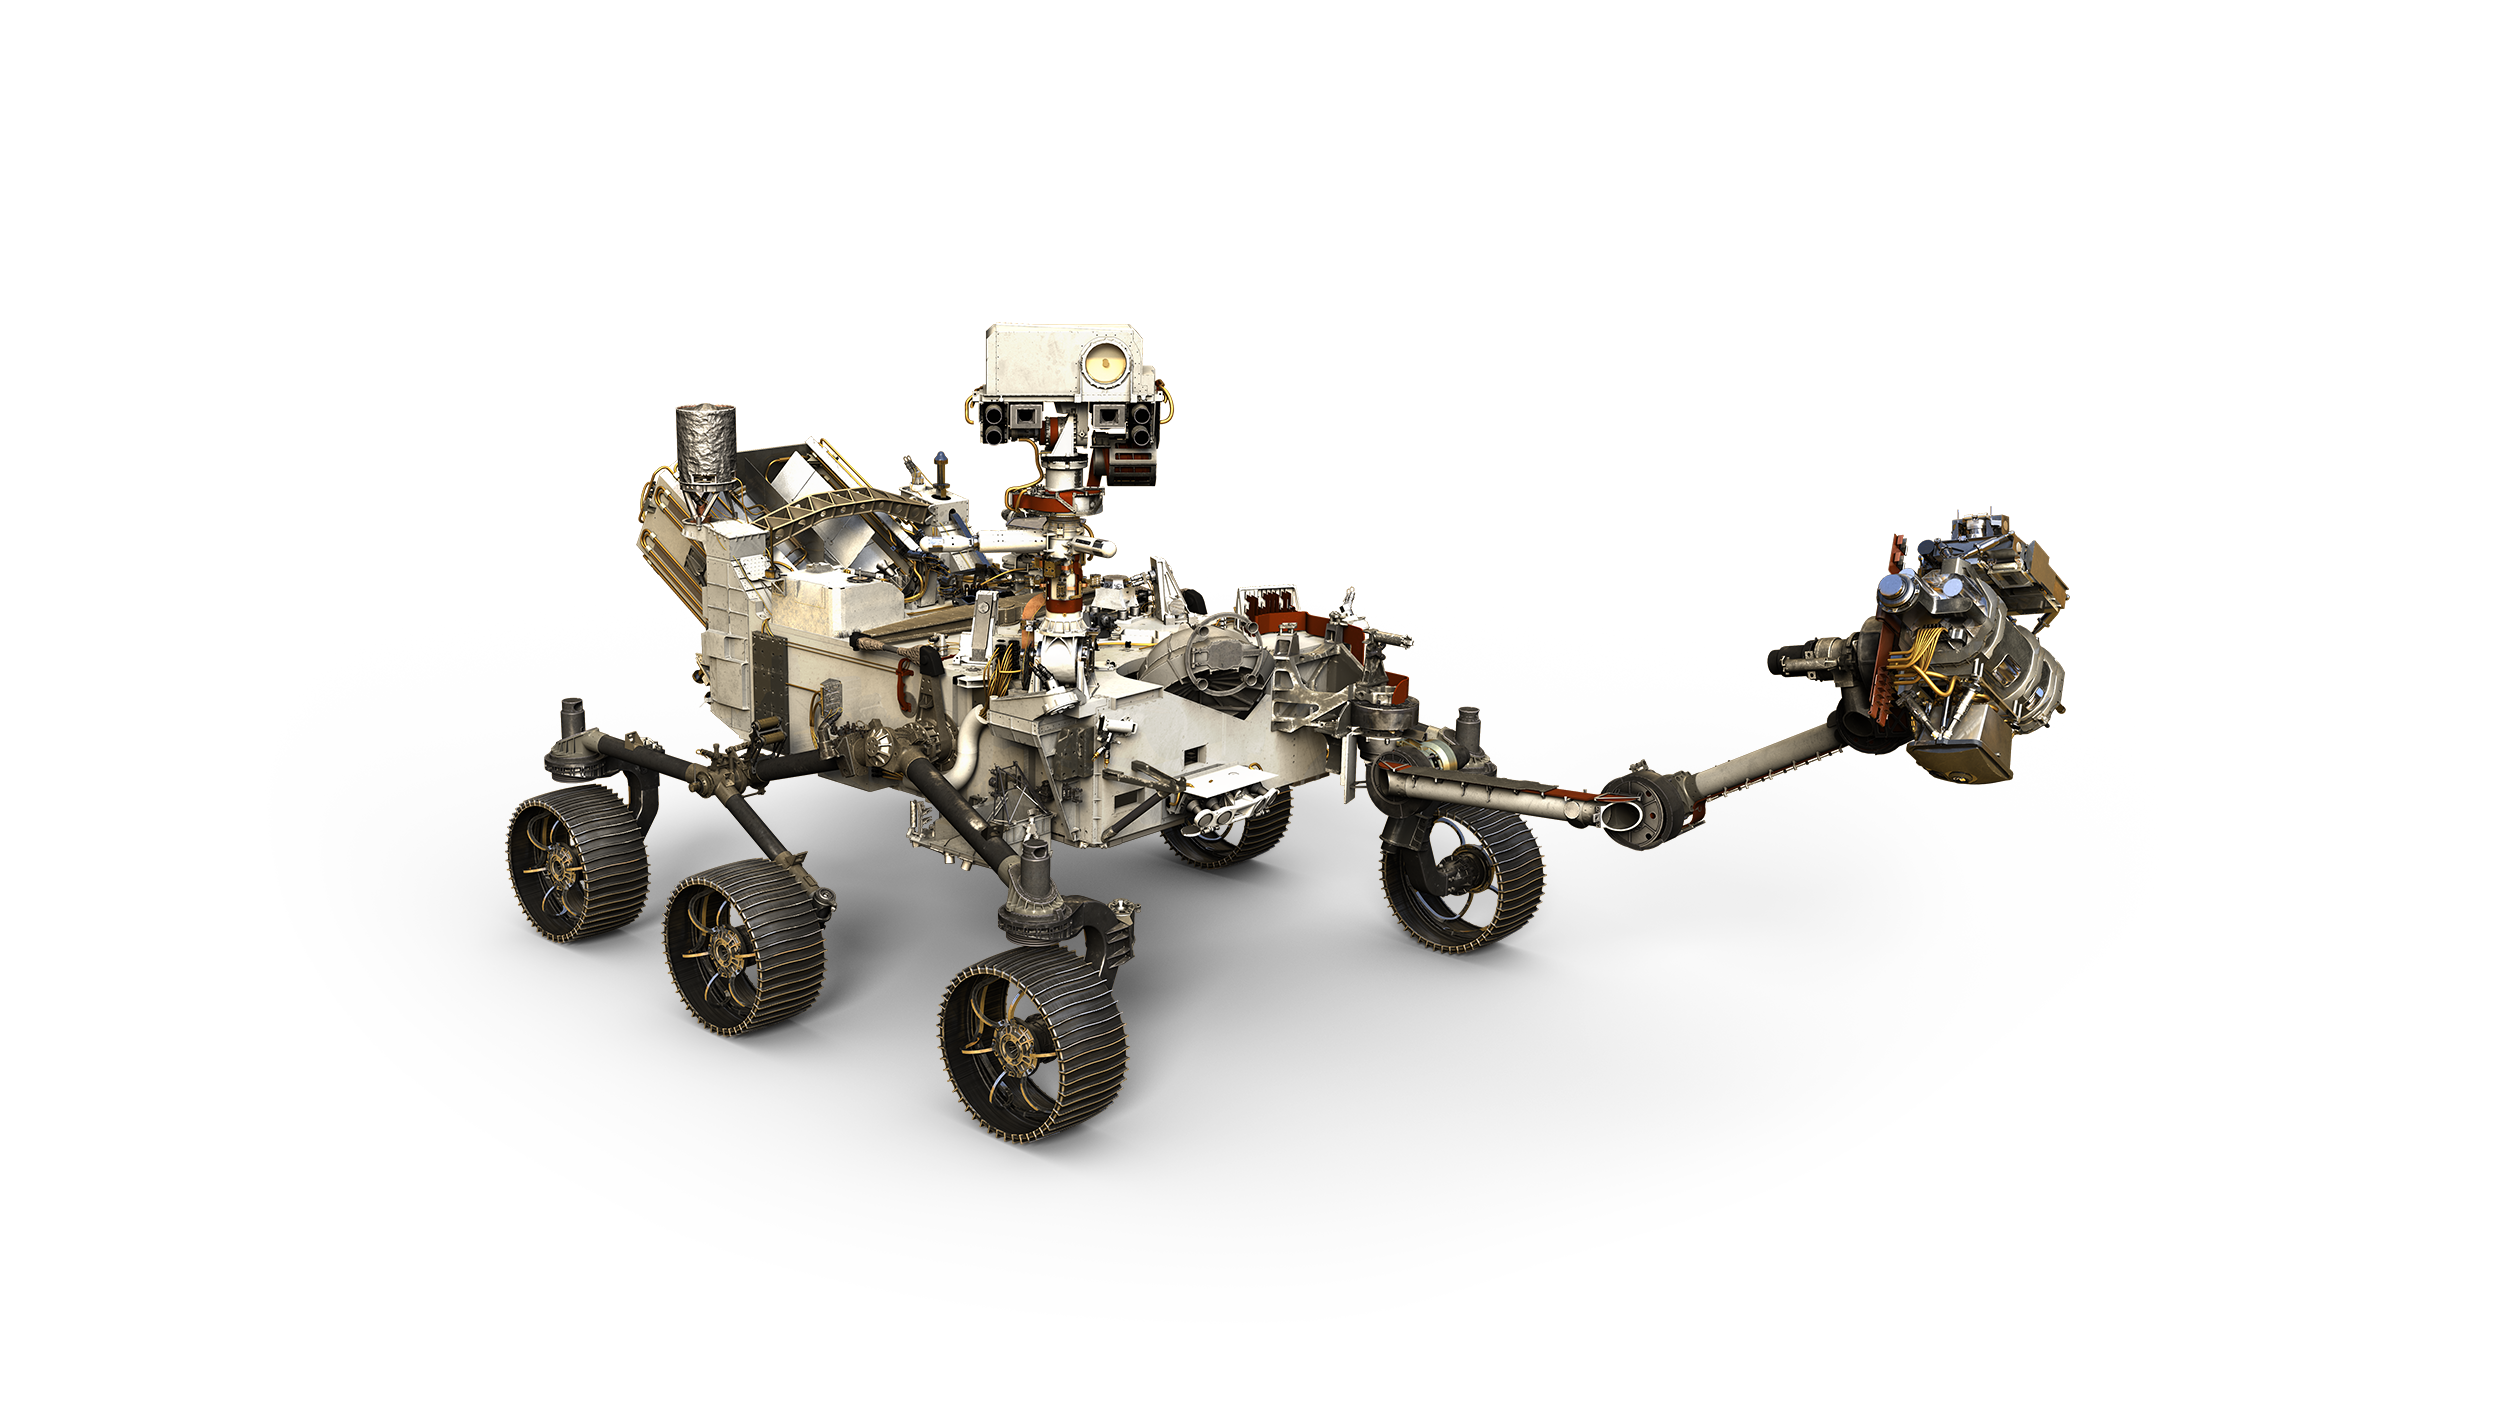
\includegraphics[scale=0.15]{JPL_rover}
	\caption{JPL Rover designed for Mars2020 mission}
\end{figure}
In industry too automated robotic systems are used in order to achieve:
\begin{itemize}
	\item A better production quality, having the possibility to more easily measure and control the performances;
	\item Improved productivity, reducing downtimes and the consumption of resources;
	\item Robots can have access to environments which are too risky or not accessible for humans;
	\item Robots maintenance can be much cheaper than other man-driven alternatives. 
\end{itemize}
In this sense mobile robotics is a very practical example of how the efficiency of a plant can be improved, reducing the effort for the trasportation tasks, or collecting datas from a warehouse automatically, or in many many other ways.\\
However, when in the early '90s people has started mounting manipulator arms on mobile platforms, the resulting system opened the research to endless possibilities. These systems are now called Mobile Manipulators.

\section{Mobile Manipulators}
The mobility of robots substantially increased what they can cope. Robots are now expected to explore unknown dynamic environments, interact with human beings or manipulate hazardous products. Mobile manipulators are systems that combine locomotion and manipulation capabilities in order to fulfil such missions. \\



Mobile manipulators can be very different, according to the environment where they are supposed to work. For example:
\begin{itemize}
	\item Submarine mobile manipulators for underwater applications;
	\begin{figure}[h!]
		\centering
		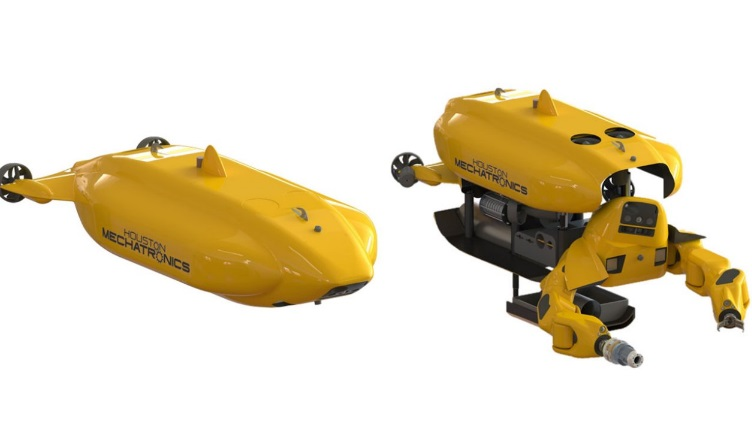
\includegraphics[scale=0.4]{submarine_robot}
		\caption{Houston Mechatronics's Aquanaut}
		\label{fig:aquanaut} 
	\end{figure}
	\item legged humanoid or animal-like robots for service missions;
	\begin{figure}[h!]
		\centering 
		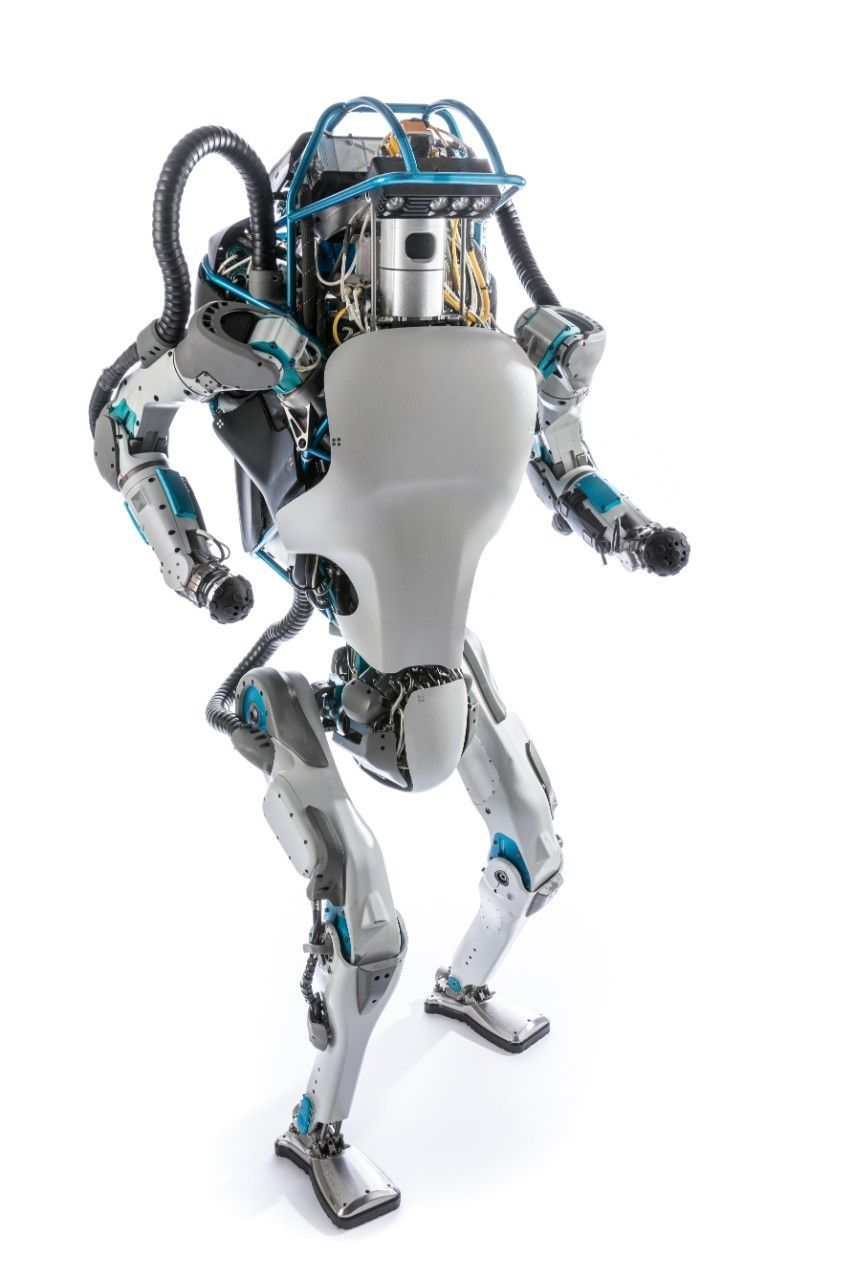
\includegraphics[scale=0.15]{atlas}
		\label{fig:atlas} 
		\quad
		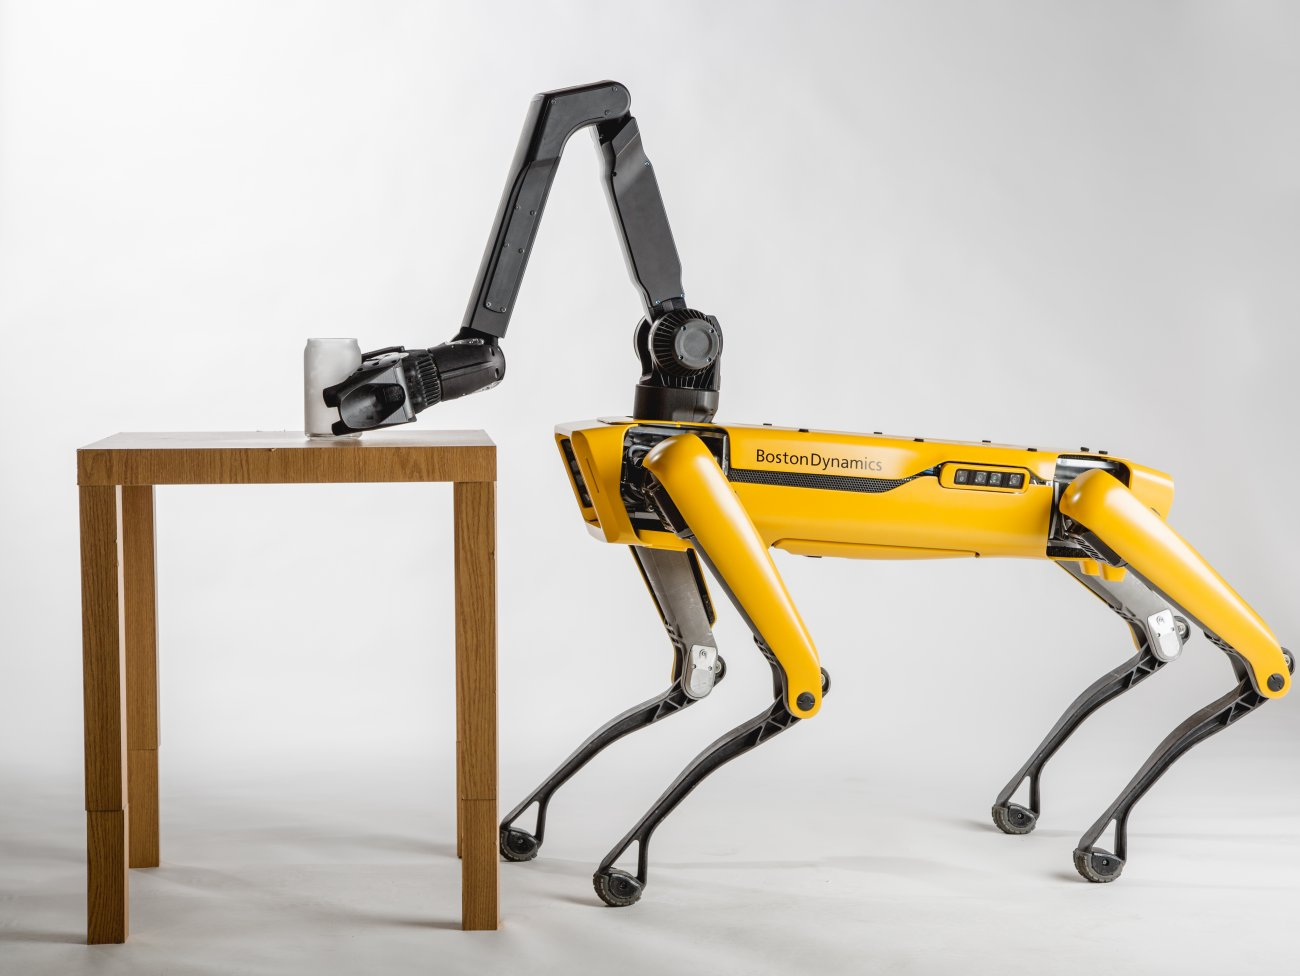
\includegraphics[scale=0.15]{spot_mini}
		\label{fig:spotmini} 
		\caption{Boston Dynamics's Atlas and Spot Mini}
	\end{figure}
	\item The most popular ones are the wheeled mobile manipulators or WMM, which combine a wheeled mobile base and one or more robotic arms.
	\begin{figure}[h!]
		\centering
		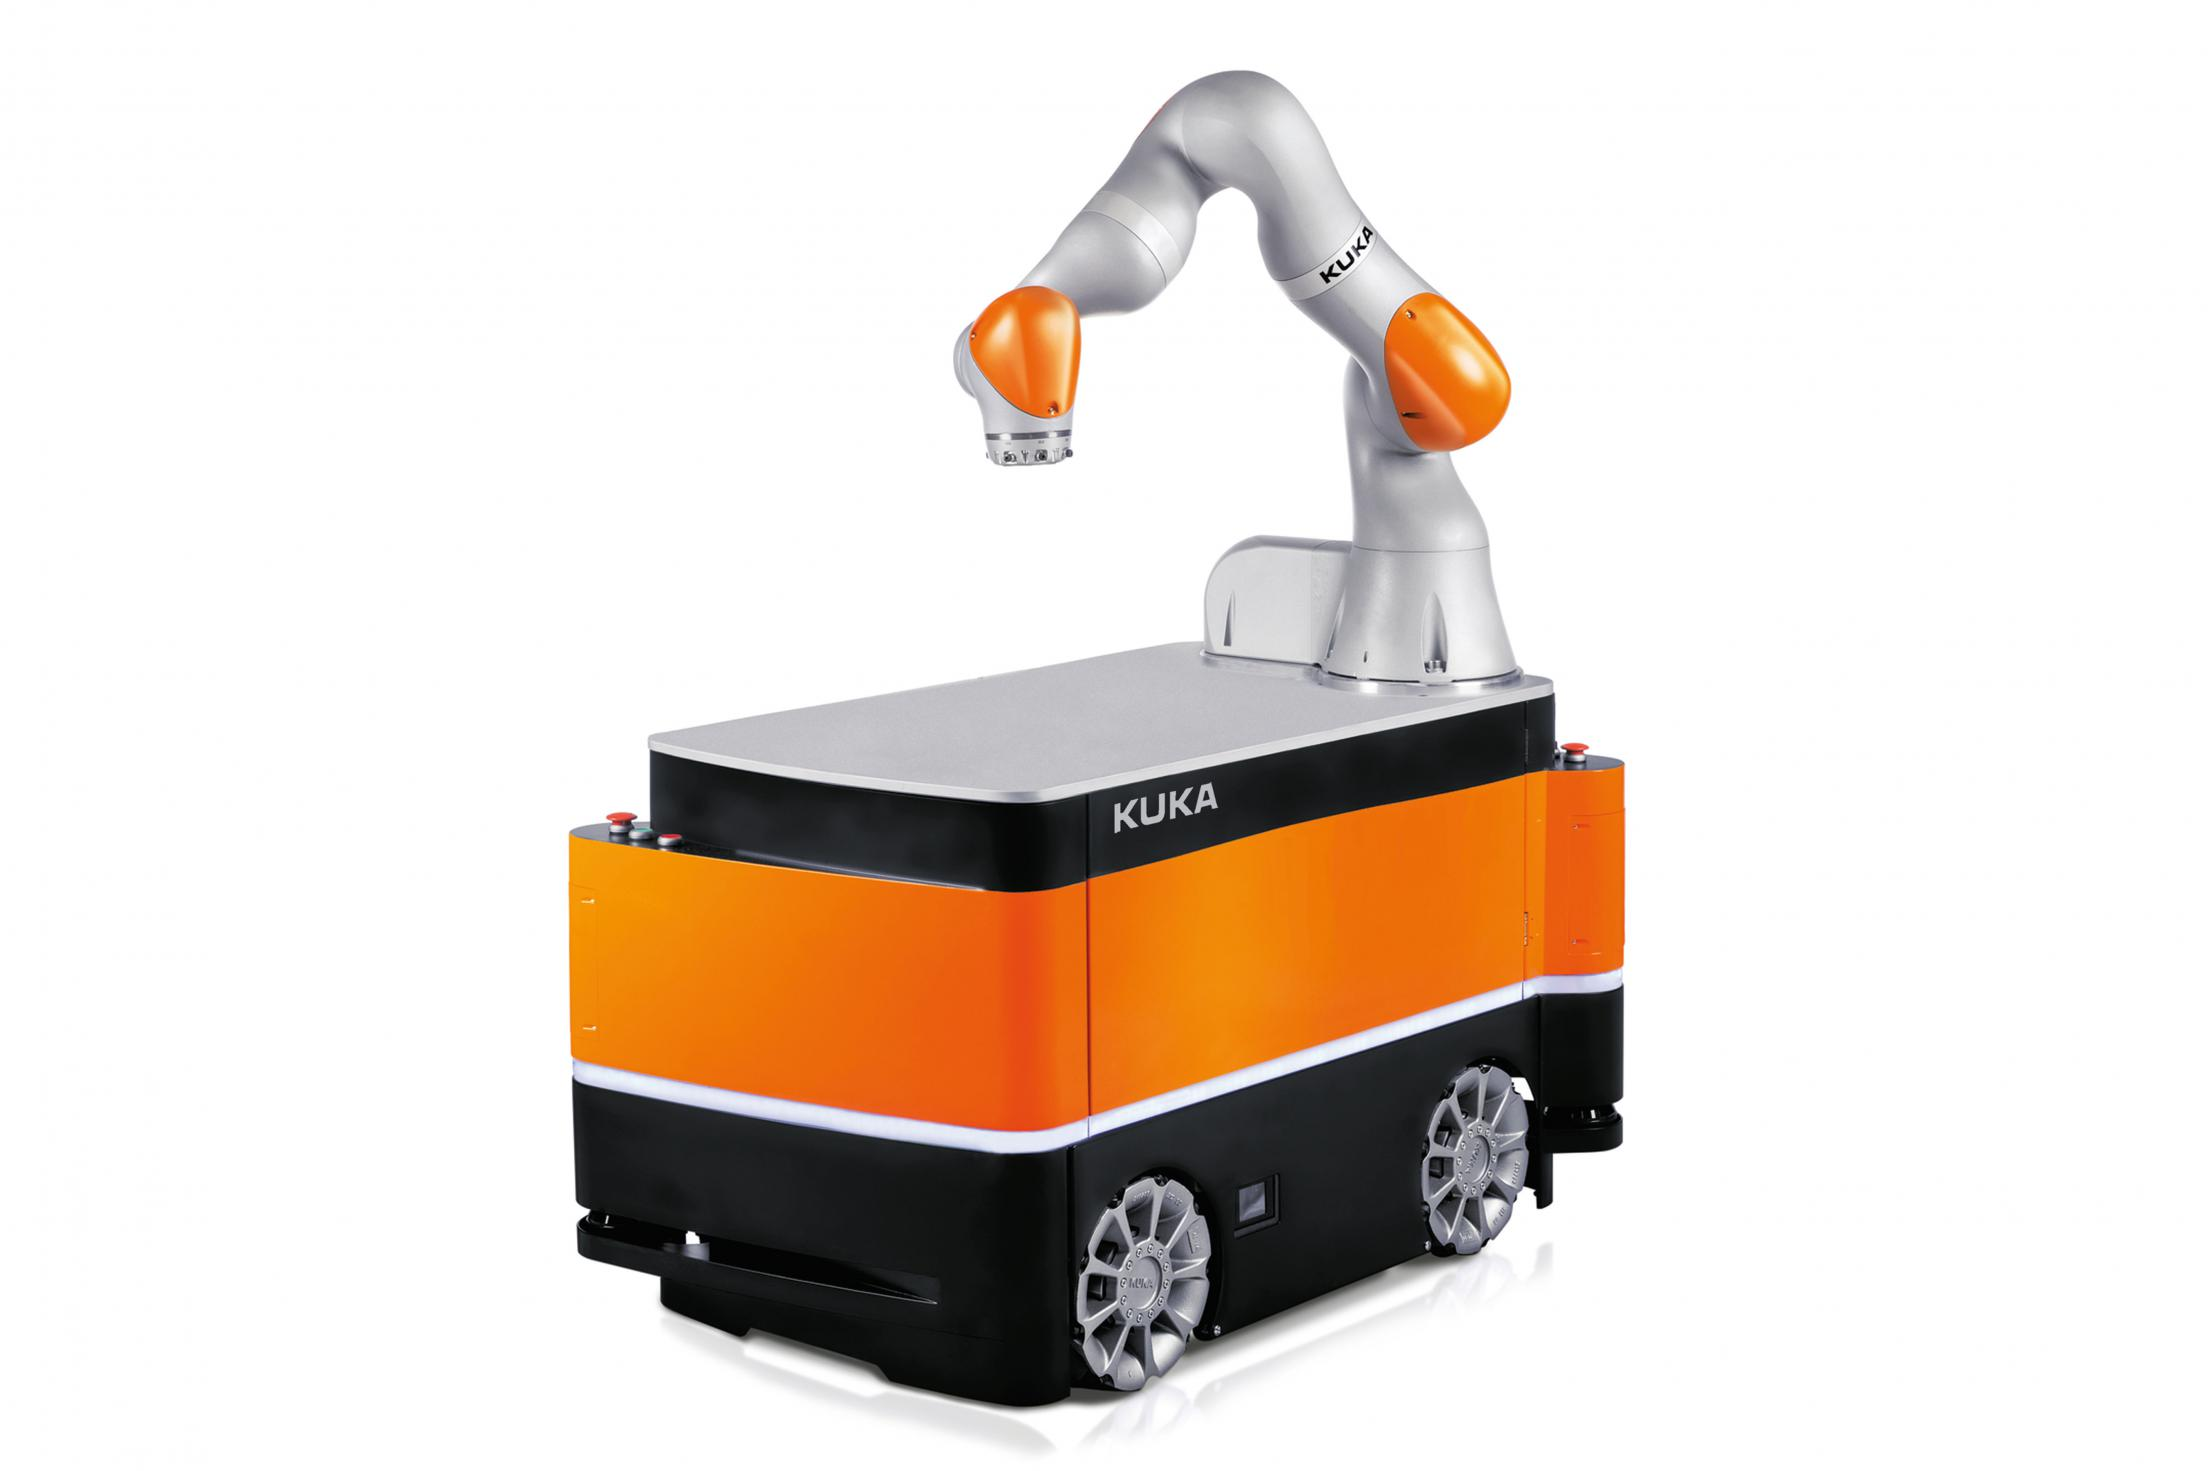
\includegraphics[scale=0.15]{kuka_iiwa}
		\caption{Kuka KMR iiwa}
		\label{fig:iiwa} 
	\end{figure}
\end{itemize}
Among the wheeled mobile manipulators there are many different types, but usually they have the following characteristics:
\begin{enumerate}
	\item The mobile base is a nonholonomic system;
	\item The entire system is often kinematically redundant with respect to the task to be achieved;
	\item The dynamic properties of the base are very different from the manipultor ones.
\end{enumerate}


\section{objective of the thesis}
\section{Achieved results}
\section{Structure of the thesis}


